\documentclass[tikz,border=4mm]{standalone}
\usepackage{amsmath,amssymb}
\usetikzlibrary{arrows.meta,calc}

\begin{document}
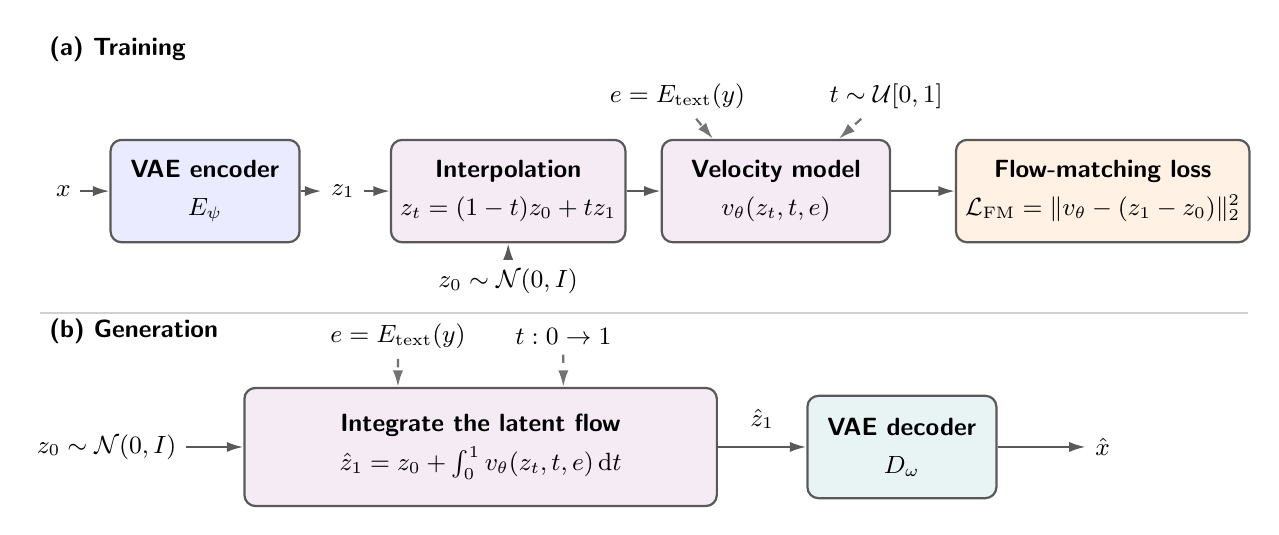
\begin{tikzpicture}[
    font=\sffamily\small,
    >={Latex[length=2.1mm,width=1.3mm]},
    data/.style={->,draw=black!65,line width=.8pt},
    condition/.style={->,dashed,draw=black!55,line width=.8pt},
    module/.style={draw=black!65,rounded corners=1.4mm,line width=.8pt,
      align=center,minimum height=13mm},
    panel/.style={font=\sffamily\bfseries\small,anchor=west},
]
  % (a) Train the latent velocity field with a frozen, pretrained VAE encoder.
  \node[panel] at (-.2,6.3) {(a) Training};

  \node (x) at (.1,4.5) {$x$};
  \node[module,fill=blue!8,minimum width=24mm] (E) at (1.9,4.5)
    {\textbf{VAE encoder}\\[1mm]$E_\psi$};
  \node (zdata) at (3.65,4.5) {$z_1$};
  \draw[data] (x) -- (E.west);
  \draw[data] (E.east) -- (zdata);

  \node (noiseTrain) at (5.75,3.35) {$z_0\sim\mathcal N(0,I)$};
  \node[module,fill=violet!8,minimum width=27mm] (interp) at (5.75,4.5)
    {\textbf{Interpolation}\\[1mm]$z_t=(1-t)z_0+t z_1$};
  \draw[data] (zdata.east) -- (interp.west);
  \draw[data] (noiseTrain.north) -- (interp.south);

  \node[module,fill=violet!8,minimum width=29mm] (velocity) at (9.15,4.5)
    {\textbf{Velocity model}\\[1mm]$v_\theta(z_t,t,e)$};
  \draw[data] (interp.east) -- (velocity.west);
  \node (textTrain) at (7.9,5.7) {$e=E_{\mathrm{text}}(y)$};
  \node (timeTrain) at (10.55,5.7) {$t\sim\mathcal U[0,1]$};
  \draw[condition] (textTrain) -- ([xshift=-8mm]velocity.north);
  \draw[condition] (timeTrain) -- ([xshift=8mm]velocity.north);

  \node[module,fill=orange!10,minimum width=34mm] (loss) at (13.3,4.5)
    {\textbf{Flow-matching loss}\\[1mm]
     $\mathcal L_{\mathrm{FM}}=\|v_\theta-(z_1-z_0)\|_2^2$};
  \draw[data] (velocity.east) -- (loss.west);

  % Panel separator.
  \draw[black!18,line width=.6pt] (-.2,2.95) -- (15.15,2.95);

  % (b) Generation requires noise, text, the learned field, and the VAE decoder.
  \node[panel] at (-.2,2.72) {(b) Generation};
  \node (noiseGen) at (.65,1.25) {$z_0\sim\mathcal N(0,I)$};
  \node[module,fill=violet!8,minimum width=60mm,minimum height=15mm] (ode)
    at (5.4,1.25) {\textbf{Integrate the latent flow}\\[1mm]
      $\hat z_1=z_0+\int_0^1 v_\theta(z_t,t,e)\,\mathrm{d}t$};
  \draw[data] (noiseGen.east) -- (ode.west);

  \node (textGen) at (4.35,2.65) {$e=E_{\mathrm{text}}(y)$};
  \node (timeGen) at (6.45,2.65) {$t:0\rightarrow1$};
  \draw[condition] (textGen) -- ([xshift=-10.5mm]ode.north);
  \draw[condition] (timeGen) -- ([xshift=10.5mm]ode.north);

  \node[module,fill=teal!9,minimum width=24mm] (D) at (10.75,1.25)
    {\textbf{VAE decoder}\\[1mm]$D_\omega$};
  \node (xhat) at (13.3,1.25) {$\hat x$};
  \draw[data] (ode.east) -- node[midway,above=1mm] {$\hat z_1$} (D.west);
  \draw[data] (D.east) -- (xhat);
\end{tikzpicture}
\end{document}
